%=============================================================================
% Traffic Digital Twin — IEEE conference report (BASE version, no Contribution)
% Compile: pdflatex report_base ; bibtex report_base ; pdflatex report_base x2
% Or upload the report/ folder to Overleaf and compile report_base.tex.
%=============================================================================
\documentclass[conference]{IEEEtran}
\IEEEoverridecommandlockouts

\usepackage{cite}
\usepackage{amsmath,amssymb,amsfonts}
\usepackage{algorithm}
\usepackage{algpseudocode}
\usepackage{graphicx}
\usepackage{booktabs}
\usepackage{textcomp}
\usepackage{xcolor}
\usepackage{tikz}
\usetikzlibrary{shapes.geometric, arrows.meta, positioning, fit, backgrounds}
\usepackage[hidelinks]{hyperref}
\usepackage{url}
\usepackage[final]{microtype}

% Long monospaced identifiers (e.g. transform.py:\_pixel\_to\_gps\_curved) cannot
% break in the narrow IEEE columns and cause large inter-word gaps. Allow a break
% after every underscore and relax justification slightly to remove the rivers.
\renewcommand{\_}{\textunderscore\allowbreak}
\setlength{\emergencystretch}{3em}

\graphicspath{{img/}{figures/}{../poster/}}

% Compile-safe figure: include the image if present (searched in figures/ and
% ../poster/ via \graphicspath), else draw a labelled placeholder. \detokenize keeps
% underscores in filenames from being read as math.
\newcommand{\figorbox}[2]{%
  \IfFileExists{img/#1}{\includegraphics[width=\linewidth]{#1}}{%
  \IfFileExists{figures/#1}{\includegraphics[width=\linewidth]{#1}}{%
  \IfFileExists{../poster/#1}{\includegraphics[width=\linewidth]{#1}}{%
  \IfFileExists{#1}{\includegraphics[width=\linewidth]{#1}}{%
    \fbox{\parbox[c][3.2cm][c]{0.92\linewidth}{\centering\small\itshape
      [figure placeholder: \texttt{\detokenize{#1}}]\\#2}}}}}}}

\begin{document}

\title{A Real-Time Traffic Digital Twin from Public CCTV:\\
Vision-Based Detection, Map-Anchored Localization, and Self-Calibrating Speed Estimation}

\author{
\IEEEauthorblockN{Minsoo Ahn}
\IEEEauthorblockA{Department of Computer Science\\
Stony Brook University\\
minsoo.ahn@stonybrook.edu}
\and
\IEEEauthorblockN{Dahyun Kwon}
\IEEEauthorblockA{Department of Computer Science\\
Stony Brook University\\
dahyun.kwon@stonybrook.edu}
}

\maketitle

%-----------------------------------------------------------------------------
\begin{abstract}
We present a real-time traffic digital twin that converts live public CCTV feeds
into an interactive, map-anchored view of road traffic. From a single clicked
camera the system streams HLS video, detects vehicles with Ultralytics YOLO26~\cite{yolo26}---an NMS-free end-to-end detector
(YOLOv8~\cite{yolov8} retained as legacy fallback)---tracks them
with a pluggable multi-object tracker (BoxMOT), and converts each vehicle's pixel
position to a geographic coordinate through a perspective homography. Because
public CCTV cameras are uncalibrated and their intrinsics are unknown, accurate
ground-plane mapping and speed estimation are the central challenges. We address
them with three complementary mechanisms: (i) a two-stage \emph{curved} transform
that maps pixels along the true road centreline obtained from the national
node-link road network rather than a flat plane; (ii) a five-stage speed estimator
combining a physics-based outlier guard, least-squares regression over a sliding
window, and per-track exponential smoothing; and (iii) a per-camera
\texttt{speed\_scale} factor that absorbs the residual geometric scale error and
is updated online via an ITS-referenced calibration loop. The system additionally
provides multi-camera background monitoring, camera-level congestion clustering,
and a SQLite time-series history with charting. We describe the architecture and
the key algorithms, and report latency, throughput, tracking-stability, and speed
metrics produced by a measurement harness over live streams.
\end{abstract}

\begin{IEEEkeywords}
digital twin, intelligent transportation systems, object detection, multi-object
tracking, homography, perspective transform, speed estimation, real-time
visualization.
\end{IEEEkeywords}

%=============================================================================
\section{Introduction}
%=============================================================================
Cities expose thousands of public traffic cameras, but the raw feeds are difficult
to interpret at scale: an operator watching a video grid cannot read off vehicle
counts, speeds, or where congestion is forming on a map. A \emph{digital twin}---a
live, geo-referenced model of the road state---turns those feeds into actionable
information. The technical obstacle is that public CCTV cameras are
\emph{uncalibrated}: their height, pitch, focal length, and exact heading are
unknown, so projecting an image detection onto the ground plane (and therefore
measuring distance and speed) is ill-posed without per-camera calibration.

This paper describes a system that ingests Korean ITS CCTV streams and produces a
real-time map-anchored twin. Our contributions, from a systems and algorithms
standpoint, are:

\begin{itemize}
  \item \textbf{Map-anchored localization.} We snap each camera onto the national
  node-link road network, extract the road centreline, and map pixels along the
  \emph{curve} of the road in two stages, rather than assuming a flat homographic
  plane. This keeps vehicle markers on the road even on bends.
  \item \textbf{Robust speed estimation without ground truth.} A five-stage filter
  (duplicate skip, physics jump guard, sliding-window least-squares regression,
  per-track exponential smoothing with spike rejection, and scale correction)
  produces stable speeds despite detection jitter and tracker ID churn.
  \item \textbf{Per-camera scale correction.} Because absolute distance scale is
  unknowable from an uncalibrated camera, the system maintains a per-camera
  \texttt{speed\_scale} that decouples geometric projection from absolute speed
  accuracy. An ITS-referenced online update loop with adaptive $\alpha$ (0.15 initially, decaying to 0.01) accumulates the factor across sessions; the current deployment has collected
  factors for 37 cameras (range 0.34--2.25), though multi-session operation is required for full convergence (see Section~\ref{sec:discuss}).
  \item \textbf{A complete, resilient pipeline.} Automatic lane-based calibration,
  manual 4-point calibration, dual-path inference (browser canvas and server-side
  HLS) over a shared detector, multi-camera background monitoring, congestion
  clustering, and a historical analytics store.
\end{itemize}

The rest of the paper is organized as follows. Section~\ref{sec:related} reviews
related work. Section~\ref{sec:design} presents the system architecture.
Section~\ref{sec:impl} details the algorithms. Section~\ref{sec:eval} reports the
measurements. Section~\ref{sec:discuss} discusses limitations, and
Section~\ref{sec:concl} concludes.

%=============================================================================
\section{Related Work}\label{sec:related}
%=============================================================================
\textbf{Object detection and tracking.} Modern traffic vision builds on real-time
detectors; we use YOLO26~\cite{yolo26} as the default detector---an NMS-free
end-to-end architecture that produces more consistent per-frame bounding-box
positions than NMS-based models such as YOLOv8~\cite{yolov8}, reducing the
ground-contact jitter that propagates into speed estimates. It also simplifies the
TensorRT FP16 engine graph (no NMS layer)~\cite{tensorrt}, lowering inference
latency and its variance; YOLOv8 is retained as a legacy fallback. For tracking we use the BoxMOT
framework~\cite{boxmot}, which exposes ByteTrack~\cite{bytetrack},
BoT-SORT~\cite{botsort}, and OC-SORT~\cite{ocsort}; appearance re-identification
uses OSNet~\cite{osnet}. Trackers without appearance ReID suffer ID switches under
occlusion, which we mitigate with a lightweight position-based ID stabilizer.

\textbf{Camera-to-ground mapping.} Mapping image points to a ground plane is a
homography problem~\cite{hartley2004}, typically solved from four correspondences
with OpenCV~\cite{opencv}. For \emph{uncalibrated} cameras, vanishing-point and
lane-geometry cues are commonly used to recover pose. Our work combines a
4-point manual mode, a vanishing-point/lane auto-calibration, and---novel in this
context---a road-centreline-following transform driven by an external road-network
dataset~\cite{moct_nodelink}.

\textbf{ITS dashboards and data.} National ITS portals~\cite{its_openapi} publish
CCTV streams and aggregated segment speeds, but typically as separate views. We
\emph{fuse} the segment speed back into the pipeline as a calibration signal.
Congestion grouping uses density-based clustering~\cite{dbscan} and convex
hulls~\cite{andrew1979}; service levels follow the Highway Capacity
Manual~\cite{los_hcm}. The visualization uses deck.gl~\cite{deckgl} over
MapLibre~\cite{maplibre}, served by FastAPI~\cite{fastapi}.

%=============================================================================
\section{System Design and Architecture}\label{sec:design}
%=============================================================================
The backend (FastAPI/Uvicorn) and a React/deck.gl frontend communicate over REST
and WebSocket. Two inference paths can produce per-frame analytics and
\emph{share a single detector}; a connection counter coordinates them so that the
multi-object tracker is never driven by two interleaved frame streams
(Fig.~\ref{fig:arch}). A two-lock scheme inside the detector
(\texttt{\_state\_lock} for tracker state, \texttt{\_lock} for GPU inference)
prevents data races between thread-pool threads, and module-level write locks
in \texttt{main.py} and \texttt{roi\_manager.py} atomize all JSON configuration
read-modify-write operations.

\begin{figure*}[t]
\centering
% --- Architecture diagram (TikZ; two-column wide, self-contained) ---
\resizebox{0.95\linewidth}{!}{%
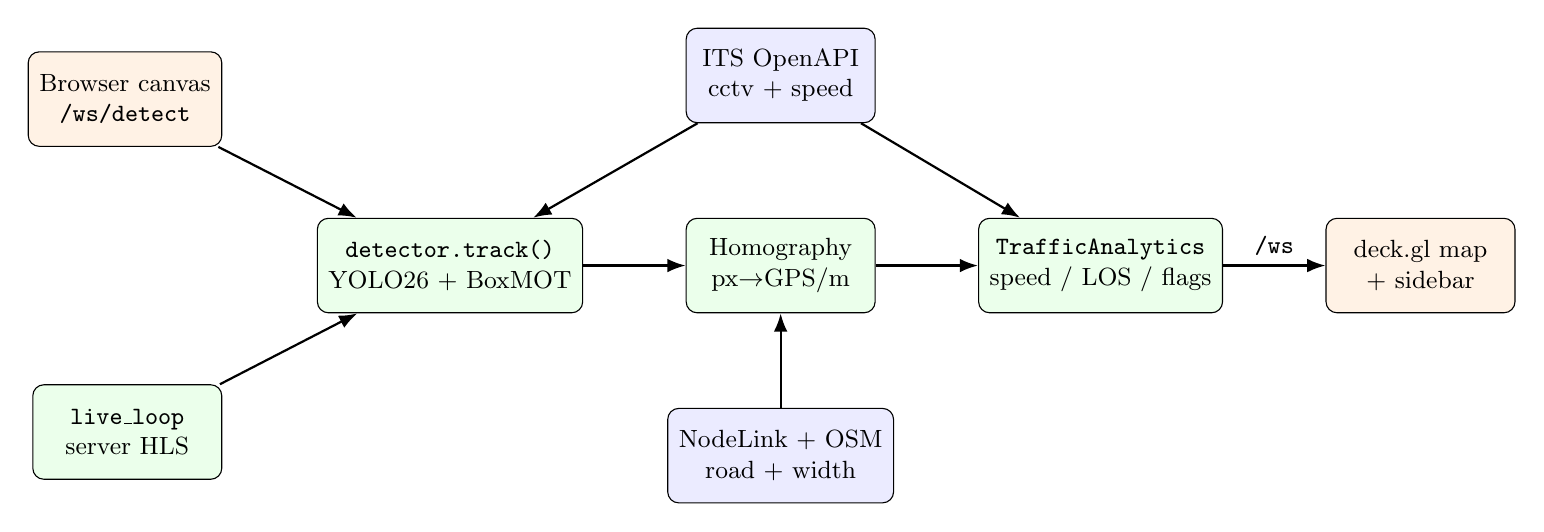
\begin{tikzpicture}[
  box/.style={draw, rounded corners, align=center, font=\small, inner sep=4pt,
              minimum height=12mm, minimum width=24mm},
  ext/.style={box, fill=blue!8},
  be/.style={box, fill=green!8},
  fe/.style={box, fill=orange!10},
  arr/.style={-{Latex}, thick}]

  % main pipeline (single row, left to right)
  \node[be] (det) {\texttt{detector.track()}\\YOLO26 + BoxMOT};
  \node[be, right=13mm of det] (tf) {Homography\\px$\to$GPS/m};
  \node[be, right=13mm of tf] (an) {\texttt{TrafficAnalytics}\\speed / LOS / flags};
  \node[fe, right=13mm of an] (ws) {deck.gl map\\+ sidebar};

  % two inputs merge into the shared detector (left side)
  \node[fe, above left=9mm and 12mm of det] (canv) {Browser canvas\\\texttt{/ws/detect}};
  \node[be, below left=9mm and 12mm of det] (live) {\texttt{live\_loop}\\server HLS};

  % external data sources (above / below the centre, short non-crossing arrows)
  \node[ext, above=12mm of tf] (its) {ITS OpenAPI\\cctv + speed};
  \node[ext, below=12mm of tf] (nl)  {NodeLink + OSM\\road + width};

  \draw[arr] (canv) -- (det);
  \draw[arr] (live) -- (det);
  \draw[arr] (det)  -- (tf);
  \draw[arr] (tf)   -- (an);
  \draw[arr] (an)   -- node[above,font=\small]{\texttt{/ws}} (ws);
  \draw[arr] (nl)   -- (tf);
  \draw[arr] (its)  -- (det);
  \draw[arr] (its)  -- (an);
\end{tikzpicture}}
\caption{System architecture. The browser path (\texttt{/ws/detect}) and the
server path (\texttt{live\_loop}) share one detector; a counter prevents concurrent
tracker calls. External data (ITS CCTV/speed, NodeLink, OSM) feeds localization and
self-calibration.}
\label{fig:arch}
\end{figure*}

\textbf{Browser path (\texttt{/ws/detect}).} The frontend plays the HLS stream
through a CORS proxy, captures canvas frames (JPEG, $\le$640\,px, $\approx$33\,ms
interval, at most two in flight), and sends them to the backend, which runs
detection, tracking, localization, and analytics, then returns an annotated frame
and broadcasts the analytics JSON to all clients.

\textbf{Server path (\texttt{live\_loop}).} The backend can also read the HLS
stream directly with OpenCV/FFmpeg and run the same pipeline. It is gated twice: it
skips tracking while a browser detection client is active (to protect the shared
tracker), and it skips all GPU work when no one is watching (the frontend reports
tab visibility). Before opening any HLS URL the detector pre-resolves HTTP\,302
redirects (\texttt{\_resolve\_hls\_url}), so FFmpeg receives a direct endpoint and
does not silently fail on delivery-layer redirect chains.

\textbf{Background services.} Periodic loops refresh expiring HLS tokens (30\,min),
poll the ITS segment speed for self-calibration (5\,min), and snapshot all monitored
cameras into a SQLite history while recomputing congestion clusters (30\,s).
To prevent the FOV polygon from flickering during auto-calibration, a slow EMA
filter stabilizes near/far distance and road-width estimates, holding the initial
accepted value fixed until sufficient samples accumulate. ROI edits trigger an
immediate GPS ring recomputation and broadcast to keep the map view synchronized.
The resulting map view is shown in Fig.~\ref{fig:map}.

\begin{figure}[t]
\centering
\figorbox{cctv_map.png}{Map view with status-coloured CCTV icons and FOV polygon}
\caption{Map view: public CCTV cameras as status-coloured icons on the vector map;
the selected camera shows its field-of-view polygon and the located vehicles.}
\label{fig:map}
\end{figure}

%=============================================================================
\section{Implementation}\label{sec:impl}
%=============================================================================

\subsection{Detection and Tracking}
The detector loads the fastest available backend---TensorRT FP16 engine, then ONNX
Runtime, then PyTorch---and exports \texttt{.pt}$\to$\texttt{.engine} on first run
when a GPU is present. A tracker \emph{tier} is chosen by GPU memory: ByteTrack
(CPU-only, no CUDA), OC-SORT (low VRAM $\ge$3.5\,GB, occlusion-robust, no ReID),
or BoT-SORT/DeepOC-SORT with OSNet appearance ReID on larger GPUs
($\ge$6\,GB and $\ge$10\,GB respectively). For the non-ReID tiers we add two robustness
layers: \texttt{\_dedup\_tracks} merges duplicate boxes (IoU\,$>$\,0.3 or centre
distance\,$<$\,40\,px, keeping the older ID), and an \texttt{IDStabilizer}
re-binds a vehicle's previous ID after a brief miss using nearest-centre matching
($\le$80\,px) with a two-pass scheme and stale-mapping purge so display IDs stay
stable and compact. Fig.~\ref{fig:yolo} shows the detection and tracking overlay.

\begin{figure}[t]
\centering
\figorbox{yolo_detect.png}{YOLO detection and multi-object tracking overlay}
\caption{Detection and tracking on a live CCTV frame: bounding boxes, vehicle class,
and stabilized track IDs.}
\label{fig:yolo}
\end{figure}

\subsection{Map-Anchored Localization}
On camera switch we query the national node-link network: we snap the camera
position perpendicularly onto the nearest road polyline, extract $\pm$150\,m of
centreline, and---because each direction is stored as a separate one-way link---we
locate the reverse carriageway and average the two snaps (when 2--40\,m apart) to
recover the true road centre. The chosen road's speed limit, lane count, and width
(\,lanes\,$\times$\,2\,$\times$\,lane-width\,) are attached to the camera; OSM
Overpass provides a width refinement when available.

Given the centreline, the \emph{two-stage curved transform} maps a pixel
$(u,v)$ to GPS along the road (Algorithm~\ref{alg:curved}).
The metric homography $H_m$ is derived from the same four image--GPS
correspondences as the GPS homography, but maps pixel coordinates to local
ENU metres rather than geographic coordinates.
Stage one maps the pixel to local metres via $H_m$; stage two decomposes the displacement
from the snap point into along-road and lateral components, advances that arc length
along the centreline, interpolates the on-road position, and re-applies the lateral
offset perpendicular to the \emph{local} road bearing. This follows real road
curvature, unlike a single flat homography.

\begin{algorithm}[t]
\caption{Two-stage curved pixel$\to$GPS transform}
\label{alg:curved}
\begin{algorithmic}[1]
\Require pixel $(u,v)$; metric homography $H_m$; snap point $p_m$ (ENU\,m);
         road bearing $b$ at snap; centreline \textit{road\_pts};
         \textit{snap\_along}; direction sign $s$
\State $(x_m,y_m) \gets H_m \cdot (u,v)$
\State $(dx,dy) \gets (x_m,y_m) - \textit{snap}_m$ \Comment{ENU from snap}
\State $d_{\parallel} \gets dx\sin b + dy\cos b;\quad d_{\perp} \gets dx\cos b - dy\sin b$
\State $\textit{arc} \gets \textit{snap\_along} + s\cdot \max(0,d_{\parallel})$
\State $(\textit{lat},\textit{lon}) \gets \textsc{InterpCenterline}(\textit{arc})$
\State $b_\ell \gets \textsc{RoadBearingAt}(\textit{arc})$
\State \textbf{apply} $d_{\perp}$ perpendicular to $b_\ell$ \Return $(\textit{lat},\textit{lon})$
\end{algorithmic}
\end{algorithm}

When no manual calibration exists, an automatic procedure estimates a homography
from one frame: Canny edges in the lower image, Hough line filtering, multi-row
sampling of left/right road edges, least-squares edge fits, vanishing-point
intersection, a pitch/height estimate from a pinhole model, and a trapezoid-to-GPS
homography. Direction (which way the camera looks along the road) is resolved by
matching the \emph{image} road-curve sign against the \emph{map} curve sign, falling
back to a vanishing-point heading test. A manual 4-point mode remains available for
maximum accuracy. Fig.~\ref{fig:calib} shows an automatic calibration result.

The primary auto-calibration path is a road-model \emph{pose solver}
(\texttt{camera\_pose.solve\_pose}): the sampled lane edges, vanishing point, and
NodeLink road width are fitted to a four-parameter pinhole-camera model ($H$,
pitch, yaw, lateral offset~$x_0$) via \texttt{scipy.optimize.least\_squares}
(soft-L1 loss). A per-row reprojection residual gates the output ($<$8\,px); on
success the solved pose is converted to four image--GPS corner pairs and used to
build both homographies. The pose is then persisted per camera to
\texttt{camera\_pose.json} so each session refines the prior, with a cold-start
fallback chain (saved prior $\to$ vehicle-bbox rough pose $\to$ GPS-grid).
A complementary \texttt{vehicle\_calib.json} accumulates a per-camera linear
pixel-to-distance model ($d = B{\cdot}y_{px} + C$, implied vanishing-point
$y_v{=}-C/B$) fitted from observed vehicle bounding-box heights; it is restored
on session start and updated online whenever sufficient samples accumulate,
providing an additional distance scale that cross-checks the geometric homography.
The trapezoid heuristic above serves only as the fallback when the residual exceeds
the quality gate or lane detection fails.

\begin{figure}[t]
\centering
\figorbox{auto_calib.png}{Automatic lane-based calibration result}
\caption{Automatic calibration: detected lane edges and the estimated vanishing point
yield the ground homography and the field-of-view footprint.}
\label{fig:calib}
\end{figure}

After GPS coordinates are assigned, a two-step post-processing pass reduces visual
noise. Per-track EMA smoothing eliminates lateral jitter while preserving along-road
motion; a jump threshold resets the filter after occlusion gaps to handle track
re-appearances correctly. A lane-offset pass then laterally separates inbound and
outbound vehicles perpendicular to the local road bearing, placing each direction on
its correct side of the road centreline for Korean right-hand traffic.

\subsection{Speed Estimation}
Speed is distance over time, and both terms are error-prone: homography distance is
noisy at the far field, and HLS buffering makes naive frame timing wrong. We use a
monotonic clock derived from stream presentation timestamps (falling back to
wall-clock), and the five-stage estimator of Algorithm~\ref{alg:speed} with the
constants in Table~\ref{tab:const}.

\begin{algorithm}[t]
\caption{Per-track speed estimation (\texttt{analytics.\_speed})}
\label{alg:speed}
\begin{algorithmic}[1]
\Require window $W$, prior EMA $v_e$, $\sigma \gets \texttt{speed\_scale}$, $\kappa \gets \texttt{depth\_corr}(y_\text{bbox})$
\State \textbf{if} duplicate position \textbf{then} skip \Comment{dedup}
\State \textbf{if} $\textit{step} > (V_{\max}/3.6\sigma)\,dt\cdot 3.0$ \textbf{then} clear $W$ \Comment{teleport reset}
\State \textbf{else if} $\textit{step} > (V_{\max}/3.6\sigma)\,dt\cdot 1.5$ \textbf{then} drop sample, keep $W$ \Comment{jump guard}
\State \textbf{if} $dt > 2$\,s \textbf{then} clear $W$ \Comment{track gap}
\State fit $\hat{v}$ by OLS on $W$ ($0.7$\,s); \textbf{if} $\mathrm{disp}(W){<}0.5$\,m \textbf{then} $\hat{v}\gets 0$ \Comment{OLS}
\State $v_e \gets (1{-}\alpha)v_e + \alpha\hat{v}\kappa\sigma$, $\alpha{=}0.35$; reject spike; decay on stop \Comment{EMA}
\State \textbf{output} $v_e$;\quad $\textit{is\_speeding} \gets \textit{reliable} \land v_e > 1.10\cdot\textit{limit}$ \Comment{output}
\end{algorithmic}
\end{algorithm}

\begin{table}[t]
\caption{Key speed/analytics constants (\texttt{config.py}).}
\label{tab:const}
\centering
\small
\begin{tabular}{@{}ll@{}}
\toprule
Parameter & Value \\
\midrule
Speed window & 0.7\,s ($W{=}\mathrm{round}(0.7\text{s}{\times}\text{FPS})$) \\
EMA $\alpha$ & 0.35 \\
Jitter threshold & 0.5 m \\
Min speed (else 0) & 5 km/h \\
Max plausible $V_{\max}$ & 180 km/h \\
GC grace & 30 frames \\
Bottleneck dwell & 150 frames ($\approx$5 s) \\
Parked dwell & 300 frames ($\approx$10 s) \\
Speeding threshold & $v_e > 1.10\times\text{limit}$ \\
LOS thresholds A--E & $\le$3,6,9,12,15 (else F) \\
Background busy & ${>}$6 vehicles \\
Background congested & ${>}$14 vehicles \\
Cluster $\varepsilon$ & 500\,m (haversine) \\
\bottomrule
\end{tabular}
\end{table}

Two additional reliability mechanisms reduce systematic bias in the speed estimate.
First, a depth-varying correction factor $\kappa$ is computed from a per-camera vehicle apparent-size model (a linear fit of inverse apparent bbox width versus vertical pixel position), compensating for the depth-dependent projection error of the homography without introducing frame-to-frame position discontinuities.
Second, vehicles whose GPS position lies more than 100\,m from the camera snap point (\texttt{SPEED\_TRUST\_MAX\_DEPTH\_M}) are flagged \texttt{speed\_reliable=False}: their speed is still displayed, but excluded from the frame average, the ITS calibration input, and speeding alerts, preventing far-field pixel noise from biasing aggregate statistics.

\subsection{Per-Camera Scale Correction}
The absolute distance scale of an uncalibrated camera is unknowable from geometry
alone, so a residual scale error persists after geometric calibration. The system
maintains a per-camera \texttt{speed\_scale} factor that multiplies the geometric
speed estimate (Algorithm~\ref{alg:speed}, line~6) and is updated online using the
ITS official segment speed as a soft reference. The ITS signal carries inherent
uncertainty---aggregated over $\approx$1\,km segments at 5-minute intervals, the
reported direction may not match the camera's field of view---so the loop adapts
slowly:
\begin{equation}
\textit{target} = \textit{scale}\cdot \frac{v_\text{ITS}}{\bar v_\text{ours}},\quad
\textit{scale} \gets \alpha\,\textit{scale} + (1{-}\alpha)\,\textit{target},
\end{equation}
with an adaptive $\alpha$ schedule and a per-update $\pm10\,\%$ step clamp in addition to the absolute $[0.3,5.0]$ bounds.
For cameras without a previously saved factor (first session), $\alpha$ decreases from $0.15$ (updates 1--2) through $0.05$ (updates 3--4) to $0.01$ thereafter, enabling fast initial convergence while damping later oscillation.
For cameras whose factor was restored from \texttt{speed\_scale.json}, $\alpha$ is fixed at $0.01$ to preserve the accumulated calibration.
The calibration uses a 10-minute rolling window of continuous, per-frame speed observations, requiring at least 50 frames with valid vehicle detections to trigger the correction, and a coefficient-of-variation guard ($\le$0.4) to skip volatile traffic.
The factor persists per camera and accumulates across sessions without resetting the geometric calibration (Section~\ref{sec:discuss}).

\subsection{Aggregation, Congestion, and History}
Direction is primarily determined by projecting each vehicle's inter-frame
displacement onto the road bearing axis with an EMA deadzone filter; a horizontal
LineZone crossing serves as a fallback when road bearing is unavailable, and also
provides In/Out counts. Dwell
counting flags bottlenecks and parked vehicles (the latter remembered by pixel
position so they survive ID changes), and a Level-of-Service grade is assigned from
the active vehicle count. Background monitoring polls additional cameras every
8\,s with detection only; cameras with more than 6 vehicles are marked \emph{busy}
and those with more than 14 are marked \emph{congested}; such cameras are then
clustered with a haversine density-based scan ($\varepsilon{=}500$\,m) and outlined
with a convex hull. A
WAL-mode SQLite store records 30\,s snapshots (14-day retention) and serves bucketed
time series, peak-time detection, and CSV export. Fig.~\ref{fig:congestion} shows the
congestion overlay.

\begin{figure}[t]
\centering
\figorbox{congestion_map.png}{Congestion overlay: CCTV icons recoloured by status}
\caption{Camera-level congestion: monitored cameras are recoloured
(normal/busy/congested) and adjacent congested cameras are grouped into a
severity-shaded region.}
\label{fig:congestion}
\end{figure}

\subsection{Visualization}
The deck.gl map layers congestion polygons, vehicle trails, the FOV polygon,
status-coloured camera icons, and vehicle markers. The FOV polygon uses one of four
strategies in priority order: (1)~the ROI GPS ring broadcast from the backend;
(2)~the manually clicked calibration ring; (3)~a straight-sided rectangle derived
from near/far distance and road width (\texttt{computeCalibPolygon}); or,
when uncalibrated, (4)~a default trapezoid.

The sidebar's vehicle list provides \emph{direction-filter tabs} (All / Inbound /
Outbound) that filter the displayed rows by the movement-vector-based direction; the
per-direction vehicle count is shown in each tab badge, and the min/avg/max speed
summary is recomputed from the filtered set. Two collapsible cards (Auto Calibration
Estimate, ITS Speed Comparison) include an info button that opens a modal explanation
of each metric, adapting to the selected map theme.

%=============================================================================
\section{Evaluation}\label{sec:eval}
%=============================================================================
Measurements are produced from the real pipeline in two ways. While the system runs
(\texttt{make dev}), an in-process collector records per-frame stage latency,
tracking, speed, and detection statistics and flushes \texttt{eval\_*.csv} and
\texttt{eval\_summary.json} every 30\,s (also on demand via \texttt{GET /eval/report});
an offline harness (\texttt{backend/evaluate.py}) reproduces the same metrics over a
live HLS source for controlled benchmarks. The system auto-selects the inference backend
(TensorRT\,$\to$\,ONNX Runtime\,$\to$\,PyTorch) and tracker tier (ByteTrack\,/\,OC-SORT\,/\,BotSort\,/\,DeepOC-SORT by GPU VRAM).

\textit{Hardware.} All timing figures are from a single machine: NVIDIA GeForce
RTX\,4070 Laptop GPU (8\,GB VRAM, compute capability 8.9), driver 610.47,
TensorRT\,10.16, ONNX\,Runtime\,1.25, Windows\,11. Absolute latency and FPS are
hardware-specific; the relative ordering across tiers and backends is the
transferable result.

\textit{Run conditions.} Model \texttt{YOLO26m}, source: National Route\,6
Namyangju Dongmakgol Intersection (live ITS HLS, nighttime), 1{,}000 frames
per run (20-frame warmup excluded). Backend and tracker are varied across runs
as shown in Tables~\ref{tab:latency} and~\ref{tab:tracker}; all other
conditions are held constant. Speed and vehicle-count figures in
Table~\ref{tab:track} are from the TensorRT\,+\,OC-SORT run and reflect
nighttime traffic at this specific location; they are included to confirm the
pipeline produces plausible output, not as ground-truth benchmarks.

\begin{table}[t]
\caption{Inference backend comparison (OC-SORT tracker fixed, 1{,}000 frames,
RTX\,4070 Laptop). Track stage includes YOLO\,+\,BoxMOT end-to-end.}
\label{tab:latency}
\centering
\small
\begin{tabular}{@{}lrrr@{}}
\toprule
Backend & Mean\,(ms) & p95\,(ms) & FPS \\
\midrule
TensorRT FP16  &  6.7 &  8.7 & 147.6 \\
PyTorch (CUDA) &  8.4 & 11.6 & 117.6 \\
ONNX Runtime   & 13.9 & 16.8 &  71.5 \\
\bottomrule
\end{tabular}
\end{table}

\begin{table}[t]
\caption{Tracker comparison (TensorRT FP16 backend fixed, 1{,}000 frames).
BoT-SORT overhead is from OSNet appearance ReID; ByteTrack shows more ID
creation events due to the absence of re-identification.}
\label{tab:tracker}
\centering
\scriptsize
\begin{tabular}{@{}lrrrrrr@{}}
\toprule
Tracker & Mean\,(ms) & p95\,(ms) & FPS & IDs & ID\,ev. & Life\,(fr.) \\
\midrule
ByteTrack &  6.6 &  7.8 & 150.9 & 27 & 286 &  35.6 \\
OC-SORT   &  6.6 &  8.9 & 150.2 &  8 &  18 &  80.0 \\
BoT-SORT  & 10.7 & 18.5 &  93.4 &  5 &  16 & 132.0 \\
\bottomrule
\multicolumn{7}{@{}l}{\scriptsize IDs = unique track IDs; ID ev. = ID creation events; Life = mean lifetime.}\\
\end{tabular}
\end{table}

TensorRT FP16 achieves the lowest latency (6.7\,ms mean), 2.1$\times$ faster
than ONNX Runtime and 1.25$\times$ faster than PyTorch on the same GPU.
ByteTrack and OC-SORT are iso-latency ($\approx$6.6\,ms), but OC-SORT's
occlusion-centric cost function reduces ID creation events from 286 to 18
and more than doubles mean track lifetime (35.6\,$\to$\,80.0 frames); BoT-SORT
adds OSNet ReID, further reducing ID events to 16 and improving lifetime to
132.0 frames at the cost of 1.6$\times$ higher latency (10.7\,ms) and a
wider p95 (18.5\,ms vs 8.9\,ms).

\begin{table}[t]
\caption{Tracking stability, speed distribution, and detection breakdown
(TensorRT\,+\,OC-SORT run, 1{,}000 frames, nighttime).}
\label{tab:track}
\centering
\small
\begin{tabular}{@{}p{0.45\linewidth}p{0.48\linewidth}@{}}
\toprule
Metric & Value \\
\midrule
Frames processed              & 1{,}000 \\
Unique tracks                 & 12 \\
Track creation events (re-entries + re-acquisitions) & 58 (4.83$\times$ unique tracks) \\
Mean track lifetime (frames)  & 124.2 \\
Median track lifetime (frames) & 131.5 \\
Max track lifetime (frames)   & 229 \\
\midrule
Vehicle speed -- mean (km/h)  & 90.9 \\
Vehicle speed -- median (km/h) & 78.2 \\
Vehicle speed -- p95 (km/h)   & 174.2$^{\dagger}$ \\
\% moving observations        & 79.6\,\% \\
Total speed observations      & 1{,}186 of 1{,}490 detections$^{\ddagger}$ \\
\midrule
Detections -- car             & 1{,}424 \\
Detections -- truck           & 66 \\
\bottomrule
\end{tabular}
\vspace{2pt}
{\footnotesize $^{\dagger}$Far-field outliers; median 78.2\,km/h is representative.\\
$^{\ddagger}$Speed requires ${\ge}W$ track-history frames; single-frame detections excluded.}
\end{table}

\textbf{Per-camera scale calibration.}
Because no per-vehicle ground truth exists for public CCTV, the system maintains a
per-camera \texttt{speed\_scale} updated online via the ITS-referenced loop.
Table~\ref{tab:scale} summarises the factors accumulated across all 37 cameras whose
streams have been monitored (\texttt{speed\_scale.json}); none had converged at
the time of writing (see Section~\ref{sec:discuss}).
The majority (51\,\%) fall within $\pm$20\,\% of 1.0, confirming that the geometric
calibration is roughly correct for most cameras; the long left tail (38\,\% below 0.8)
reflects cameras with steep pitch or far-field observation zones that compress apparent
displacement, while the small right tail (11\,\% above 1.2) corresponds to
wide-angle or low-mounted cameras that exaggerate it.

\begin{table}[t]
\caption{Distribution of learned \texttt{speed\_scale} factors across 37 cameras
(\texttt{speed\_scale.json}). Values below~1.0 indicate geometric underestimation
of displacement (common when the camera axis is oblique to the road); values
above~1.0 indicate overestimation. All factors are unconverged at this snapshot.}
\label{tab:scale}
\centering
\small
\begin{tabular}{@{}lrr@{}}
\toprule
Range & Cameras & Share \\
\midrule
$<0.5$          &  4 & 10.8\,\% \\
$0.5$--$0.8$    & 10 & 27.0\,\% \\
$0.8$--$1.2$    & 19 & 51.4\,\% \\
$>1.2$          &  4 & 10.8\,\% \\
\midrule
\multicolumn{3}{@{}l}{Min / Max: 0.34\,/\,2.25} \\
\multicolumn{3}{@{}l}{Mean / Median: 0.90\,/\,0.85} \\
\bottomrule
\end{tabular}
\end{table}

%=============================================================================
\section{Discussion and Limitations}\label{sec:discuss}
%=============================================================================
The homography is accurate inside the calibration quadrilateral and extrapolates
with growing error toward the far field; we mitigate this with the dual-matrix
calibration, the regression window, and lane-based auto-calibration, but a
residual error remains on poorly observed cameras.
Automatic calibration assumes a focal length of $1.2\times$ image height (unknown
intrinsics), giving a $\pm$15--20\,\% scale uncertainty per FoV mismatch. It also
fails when lane markings are not visible (night, rain, dense traffic), falling back
to an approximate grid.
Road width is inferred from lane count and assumed bidirectional, so one-way roads
are over-wide. The nearest node-link road is occasionally the wrong one (e.g., a
camera near both a national route and an expressway), which displaces the FOV
polygon and vehicle GPS; the CCTV-name road-hint reduces but does not eliminate this.
Finally, congestion is clustered at the camera level because background cameras
expose only counts, not per-vehicle speeds.

The ITS-based self-calibration loop uses an adaptive learning rate (0.15 on the first two updates, decaying to 0.01 after convergence, every 5\,min) to treat the ITS segment speed as an imprecise soft reference, since ITS figures reflect 1-km road-segment averages that may not align with the camera's exact observation zone or direction.
The adaptive schedule accelerates initial convergence for new cameras while preserving accumulated corrections for returning ones, but multi-session operation is still required for the factor to fully stabilize; none of the 37 accumulated cameras had converged at time of evaluation. The scale factors therefore capture the geometric projection bias present at each camera and should be interpreted as a running estimate rather than a definitive calibration.

Because the system derives all geographic positions from map geometry rather than
on-vehicle GPS receivers, localization accuracy is bounded by the quality of the
NodeLink road database and the precision of the perspective projection; errors in
map alignment or road-shape approximation propagate directly into vehicle GPS
coordinates. Additionally, a camera's effective field of view is strongly shaped by
its mounting angle: a steeply pitched installation sees a narrow, elongated strip of
road, producing a thin FOV polygon on the map and limiting the usable observation
window even after geometric calibration.

A structural limitation is the system's dependence on national ITS
infrastructure: camera streams and segment speeds are fetched from a
government-operated open API~\cite{its_openapi} whose availability and
authentication policy are outside the operator's control and may be
restricted or discontinued. Camera placement and viewing angle are fixed by
road authorities and cannot be adjusted; some installations are positioned
too far or too close to capture a useful road segment, and extreme viewpoints
cannot be recovered through calibration. Adverse conditions---low
illumination, rain, lens contamination, and hardware faults---can suppress
the visual signal entirely, leaving the pipeline with no basis for detection
or calibration. These constraints are inherent to re-using existing
infrastructure without modification.

%=============================================================================
\section{Conclusion}\label{sec:concl}
%=============================================================================
We built a real-time traffic digital twin that localizes vehicles on a map from
uncalibrated public CCTV and estimates their speed without ground truth. The key
ideas are a road-centreline-following two-stage transform, a robust five-stage speed
estimator, and a per-camera scale-correction framework with an ITS-referenced online
update loop, wrapped in a resilient dual-path pipeline with congestion analytics and
a historical store. The automatic calibration pipeline---geometric pose solver plus
the accumulating scale factor---substantially reduces the per-camera manual setup
required to deploy across many cameras, while the system remains operational even
before the ITS loop converges.

A distinguishing property is that the system requires \emph{no GPS instrumentation
on vehicles}: conventional traffic monitoring relies on embedded GPS loggers or
dedicated roadside sensors, both of which demand significant infrastructure
investment. By re-purposing cameras that road authorities already operate, the
system tracks multiple vehicle classes simultaneously across multiple views with no
additional hardware cost. As public CCTV coverage continues to expand and object
detectors advance, this class of vision-only traffic twin becomes increasingly
practical at scale. With wider network integration, the same localization
principle---positioning objects through perspective projection rather than satellite
signal---could extend to GPS-denied environments such as tunnels, underground
parking, and indoor logistics facilities; the per-camera track-ID scheme further
enables cross-camera vehicle re-identification for a range of fleet management and
security applications.

%=============================================================================
\bibliographystyle{IEEEtran}
\bibliography{refs}

\end{document}
